\documentclass{article}
% The LaTeX macro language is complicated, so we have inserted
% lots of documenting comments into the file.  Comments start
% with `%' and continue to the end of the line.  In Overleaf's
% window, they are colored green
%
% Comments prefixed with `Student:' are relevant to students.
% Skip anything else you don't understand, or ask me.
%
% set font encoding for PDFLaTeX or XeLaTeX
\usepackage{ifxetex}
\ifxetex
  \usepackage{fontspec}
\else
  \usepackage[T1]{fontenc}
  \usepackage[utf8]{inputenc}
  \usepackage{lmodern}
\fi

% Student: These lines describe some document metadata.
\title{Problem Set 6}
\author{%
% Student: change the next line to your name!
    Name
\\  MATH-UA 120 Discrete Mathematics
}
\date{due November 10, 2023}


\usepackage[headings=runin-fixed-nr]{exsheets}
% These make enumerates within questions start at the second ("(a)") level, rather than the first ("1.") level.
\makeatletter
    \newcommand{\stepenumdepth}{\advance\@enumdepth\@ne}
\makeatother
\SetupExSheets{
    question/pre-body-hook=\stepenumdepth,
    solution/pre-body-hook=\stepenumdepth,
}
\DeclareInstance{exsheets-heading}{runin-nn-np}{default}{
    runin = true,
    title-post-code = .\space,
    join = {
        main[r,vc]title[l,vc](0pt,0pt);
    }
}
\newif\ifshowsolutions
% Student: replace `false' with `true' to typeset your solutions.
% Otherwise they are ignored!
\showsolutionstrue
\ifshowsolutions
    \SetupExSheets{
        question/pre-hook=\itshape,
        solution/headings=runin-nn-np,
        solution/print=true,
        solution/name=Answer
    }%
    \makeatletter%
    \pretocmd{\@title}{Answers to }%
    \makeatother%
\else
    \SetupExSheets{solution/print=false}
\fi

% Bug workaround: http://tex.stackexchange.com/a/146536/1402
%\newenvironment{exercise}{}{}
\RenewQuSolPair{question}{solution}
%\let\answer\solution
%\let\endanswer\endsolution
\usepackage{manfnt}
\newcommand{\danger}{\marginpar[\hfill\dbend]{\dbend\hfill}}

% We are creating a command for some common commands.
\newcommand{\Z}{\mathbb{Z}}
\newcommand{\N}{\mathbb{N}}
\newcommand{\R}{\mathbb{R}}
\newcommand{\im}{\operatorname{im}}
\newcommand{\id}{\operatorname{id}}

% This package is for specifying graphics.  It's amazing.
% Manual at http://texdoc.net/texmf-dist/doc/generic/pgf/pgfmanual.pdf
\usepackage{tikz}

\usepackage{amsmath, amsthm}
\usepackage{amsfonts}
\usepackage{siunitx}
\DeclareSIUnit\pound{lb}
\usepackage{hyperref}
\newtheorem*{theorem}{Theorem}
\theoremstyle{definition}
\newtheorem*{definition}{Definition}
% This is the beginning of the part of the file that describes
% the text of the document.
% That's why it says `\begin{document}' below. :-)
\begin{document}
\maketitle



These are to be written up in \LaTeX{} and turned in to Gradescope.\\



\ifshowsolutions
    \SetupExSheets{solution/print=true}
\else
    \danger
 \underline{ \LaTeX{}  Instructions:}  You can view the source (\texttt{.tex}) file to get some more examples of \LaTeX{} code.  I have commented the source file in places where new \LaTeX{} constructions are used.
  
  Remember to change \verb|\showsolutionsfalse| to \verb|\showsolutionstrue|
    in the document's preamble 
    (between \verb|\documentclass{article}| and \verb|\begin{document}|)
\fi

\section*{Assigned Problems}


\begin{question}
    Suppose that we have two piles of cards each containing $n$ cards. Two players play a game as follows. Each player, in turn, chooses one pile and then removes any number of cards, but at least one, from the chosen pile. The player who removes the last card wins the game. Show that the second player can always win the game.
\end{question}
% Student: put your answer between the next two lines.
\begin{solution}
	\begin{description}
	\item[Base Cases: ] Consider $n=1$. The first player removes one card from either pile. The second player then removes the last card and wins the game.
	
	\item[Inductive Hypothesis: ] Suppose that $k\geq 1$ and whenever there are two piles of $n$ cards for $1\leq n\leq k$, the second player can always win the game.
	
	\item[Inductive Step: ] Suppose there are two piles of $n=k+1$ cards. The first player removes $i$ cards from one of the piles, where $1\leq i\leq k+1$. 
	\begin{itemize}
	\item If $i=k+1$ (i.e. the first player removes all of the cards from one pile), the second player can win by removing all of the cards from the remaining pile. 
	\item If $i<k+1$, the second player removes $i$ cards from the other pile leaving two piles each with $k+1-i$ cards. The game then resumes with the first player facing two piles each with $k+1-i<k+1$ cards. By the inductive assumption, the second player can win the game.
	\end{itemize}
	\end{description}
	Therefore, by strong induction, the second player can always win the game.
	
{\color{red} Rubric:
\begin{itemize}
\item Follow RVF rubric with 1P for \LaTeX
\end{itemize}}
\end{solution}


\begin{question}
    For each of the following functions, say if it is one-to-one and / or onto? Prove or disprove each statement.
    \begin{enumerate}
	\item $f : \Z \to \Z$ with $f(n) = n^2 + 1$ for $n \in \Z$.
	\item $f : \Z \to \Z$ with $f(n) = n/2$ if $n$ is even, and $f(n) = 0$ if $n$ is odd.
	\item $f : \R \to \R$ with $f(x) = 1/x$ if $x \neq 0$, and $f(0) = 0$.
	\item $f: \N \to \N$ with $f(n) = 2^n$ if $n$ is even and $f(n) = n$ if $n$ is odd.
	\item $f : \mathcal{P}(\Z) \to \mathcal{P}(\Z)$ with $f(A) = A \cup \{ 0 \}$ for $A \in \mathcal{P}(\Z)$.
    \end{enumerate}
\end{question}
% Student: put your answer between the next two lines.
\begin{solution}
\begin{enumerate}
	\item $f$ is not 1-1 since $f(-1) = f(1) = 2$. $f$ is not onto since $f(n) \geq 1$ for all $n$ so we cannot find a $n \in \Z$ s.t. $f(n) = 0$.
	
	\item $f$ is not 1-1 since $f(0) = f(1) = 0$. $f$ is onto since for $m \in \Z$, we have $f(2m) = 2m/2 = m$.
	
	\item
	\begin{itemize}
		\item $f$ is 1-1. Take $x, y \in \R$ and assume $f(x) = f(y)$. Then either $x$ and $y$ are both nonzero, and then this means that $1/x = 1/y$ and thus $x = y$. Or one of them is zero, but then $f(x) = f(y) = 0$, which can only happen when $x = y = 0$.
		\item $f$ is onto. Take $y \in \R$. If $y = 0$, then $f(0) = y$. Otherwise, $f(1/y) = 1/(1/y) = y$.
	\end{itemize}
	
	\item 
	
	\begin{itemize}
		\item $f$ is not 1-1 since $f(0) = 2^0 = 1 = f(1)$.
		
		\item $f$ is not onto. Indeed, $f(n)$ is either a power or 2 or is odd, so for instance, we cannot find $n$ such that $f(n) = 0$.
		
	\end{itemize}
	
	\item $f$ is not 1-1 since $f(\emptyset) = f(\{0 \}) = \{ 0 \}$. $f$ is not onto since by definition, for any $A \in \mathcal{P}(\Z)$, $f(A)$ contains 0, so for instance, there cannot be a $A$ such that $f(A) = \emptyset$.
	
\end{enumerate}

{\color{red} Rubric:
\begin{itemize}
\item 2P each
\end{itemize}}
\end{solution}




\begin{question}
    \begin{enumerate}
        \item Let $A = \{1,2,3,4\}$ and $B = \{5,6,7\}$.
        Let $f$ be the relation $ \left\{(1,5),(2,5),(3,6),(?,?)\right\} $ where the question marks are to be filled in by you. 
        Give an example of $(?,?) \in A \times B$ so that: (Remember to explain your reasoning.)
            \begin{enumerate}
                \item The relation $f$ is not a function.
                \item The relation is a function from $A$ to $B$ but not onto $B$.
                \item The relation is a function from $A$ to $B$ and is onto $B$.
            \end{enumerate}

        \item     Let $A$ be an $n$-element set and let $i, j, k \in \mathbb{N}$ with $i+j+k = n$.
        How many functions $f \colon A \to \{0,1,2\}$ are there for which all three of the below are satisfied:
            \begin{itemize}
                \item $\left|\left\{ a \in A : f(a) = 0 \right\} \right| = i$
                \item $\left|\left\{ a \in A : f(a) = 1 \right\} \right| = j$
                \item $\left|\left\{ a \in A : f(a) = 2 \right\} \right| = k$
            \end{itemize}
    \end{enumerate}
\end{question}
% Student: put your answer between the next two lines.
\begin{solution}
\begin{enumerate}
	\item 
	\begin{enumerate}
		\item Take $(?,?) = (3,5)$, for example. Then the relation $f$ is not a function since  otherwise the function would take two different values on $3$.
		\item Take $(?,?) = (4,5)$, for example. Then the relation $f$ is a function since it is well defined for every value of $A$,  but it is not onto $B$ since the value $7\in B$ is never attained. 
		\item Take $(?,?) = (4,7)$, for example. Then the relation $f$ is a function since it is well defined for every value of $A$,  and it is onto $B$ since each value of $ B$ is attained for some value of $A$. 
	\end{enumerate}

	\item      To construct such a function, we first choose $i$ elements to send to $0$.
	There are $\binom{n}{i}$ ways to do this.  Then we choose $j$ of the remaining
	$n-i$ elements to send to $1$.  There are $\binom{n-i}{j}$ ways to do this.
	The remaining $n-i-j = k$ elements are sent to $2$.  So the total number
	of functions is
	\[
	\binom{n}{i} \binom{n-i}{j}
	= \frac{n!}{i!(n-i)!} \cdot \frac{(n-i)!}{j!(n-i-j)}
	= \frac{n!}{i!\,j!\,k!}
	\]

\end{enumerate}
{\color{red} Rubric:
\begin{itemize}
\item part a: 2P each
\item part b: 2P for answer and 2P for explanation
\end{itemize}}


\end{solution}

\begin{question}
    \begin{enumerate}
	\item There are five points inside an equilateral triangle of side length 2. 
	Show that at least two of the points are within 1 unit distance from each other.
	\item Let $A$ be a set of 10 distinct integers between 1 and 100 (both inclusive). 
	Show that there are two nonempty and disjoint subsets of $A$ such that the sum of all its elements are the same.
    \end{enumerate}
\end{question}
% Student: put your answer between the next two lines.
\begin{solution}
\begin{enumerate}
	\item 	
	Divide the given equilateral triangle of side length 2 into four unit triangles (``holes'').  If we have five points (``pigeons'') inside the given equilateral triangle, then by pigeonhole principle there will be one unit triangle that contains at least two of the points.  Since this triangle has side length 1, then the distance between these two points is less than or equal to 1.  So, two of the points are within one unit distance from each other.
		{\color{red}
		\begin{center}
			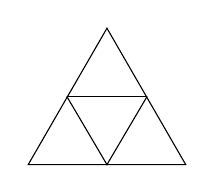
\begin{tikzpicture}
				\coordinate (A) at (-1, 0);
				\coordinate (B) at (0, 0);
				\coordinate (C) at (1, 0);
				\coordinate (D) at (0, 1.732);
				\coordinate (E) at (-.51, .866);
				\coordinate (F) at (.51, .866);
				\draw (A) -- (C) -- (D) -- cycle;
				\draw (E) -- (B) -- (F);
				\draw (E) -- (F);
			\end{tikzpicture}
	\end{center}}


	\item Note that it is enough to find two nonempty different subsets having the same sum: by subtracting their intersection, we get two nonempty disjoint subsets whose elements have the same sum. Remember, \textit{different sets} and \textit{disjoint sets } does not mean the same thing. For example, $\{1,5,4\}$ and $\{6,4\}$ are not disjoint but they have the same sum. Take away their intersection, you're left with both sets having the same sum. (You can easily generalize this argument). 
	
	
	The number of nonempty subsets of $A$ is $2^{10}-1 = 1023$. We also eliminate the case where the subset of $A$ is the entire set $A$ since if that happens to be a subset, we are left with the empty set as the other set. Thus, we have 1022 subsets of interest for us here, which will contain at least 1 element and at most 9 elements.
	
	 The sum of the elements of such a subset is at least equal to 1 (when one subset is just $\{1\}$) and at most $ 92 + ... + 100 = 864$ (when one subset consists of those numbers). There are therefore more subsets of interest for us here than possible sums. By the pigeonhole principle, there are at least two nonempty and different subsets of $A$ that have the same sum.
	 
\end{enumerate}

{\color{red} Rubric:
\begin{itemize}
\item 5P each:
\item 3P: Explanation for how to break things up
\item 2P: Argue pigeonhole principle
\end{itemize}}
\end{solution}


\begin{question}
    Let $A = \{ x \in \Z ~:~ 3|x \}$.  Show that $A$ and $\mathbb{N}$ has the same cardinality.  {\it Hint:} Define $f: A \rightarrow \N$ such that
\[ f(x) =\left\{\begin{array}{c c l} \frac{2}{3}x & & \text{if } x \geq 0 \\ ~ \\ -\frac{2}{3}x - 1 &  & \text{if } x < 0 \end{array} \right. .\]
\end{question}
% Student: put your answer between the next two lines.
\begin{solution}
Let $f: A \rightarrow \N$ such that 
\[ f(x) =\left\{\begin{array}{c c l} \frac{2}{3}x & & \text{if } x \geq 0 \\ ~ \\ -\frac{2}{3}x - 1 &  & \text{if } x < 0 \end{array} \right. .\]
(Note that if $x \geq 0$, then $f(x)$ is even and if $x < 0$, then $f(x)$ is odd.)

\begin{itemize}
\item We show that $f$ is one-to-one:\\
Suppose that for $a, a' \in A$, $f(a) = f(a')$.  If $f(a) = f(a')$ is even, then
\begin{eqnarray*}
f(a) & = & f(a') \\
\frac{2}{3} a & = & \frac{2}{3} a' \\
a & = & a' \hspace{1cm} \text{ divide both sides by } 2/3.
\end{eqnarray*}
If $f(a) = f(a')$ is odd, then
\begin{eqnarray*}
f(a) & = & f(a') \\
-\frac{2}{3} a - 1 & = & -\frac{2}{3} a' - 1 \\
-\frac{2}{3} a & = & -\frac{2}{3} a'\hspace{1cm} \text{ add 1 to both sides }\\
a & = & a' \hspace{1cm} \text{ divide both sides by } -2/3.
\end{eqnarray*}
So, $f$ is one-to-one.
\item We show that $f$ is onto:\\
Suppose that $n \in \N$ is even, then let $a = \frac{3n}{2}$.  Then, since $a \geq 0$, 
\[ f(a) = f(3n/2) = \frac{2}{3} \frac{3n}{2} = n. \]
If $n \in \N$ is odd, then let $a = -\frac{3(n+1)}{2}$.  Since $a < 0$,
\[ f(a) = f(-3(n+1)/2) = -\frac{2}{3}\left(-\frac{3(n+1)}{2}\right) - 1 =  n+1 - 1 = n.\]
So, $f$ is onto.

\end{itemize}
{\color{red} Rubric:
\begin{itemize}
\item 5P for 1-1
\item 5P for onto
\end{itemize}}
\end{solution}





\end{document}
